\subsection{Immediate Feedback}
\label{bretvictor}

After having introduced the notion of immutable data and its advantages
in systems design but also the usefulness of state and
where it can be a viable tool, the last piece that is needed in order
to introduce the \textit{Drift} project is how to interface with
the user.

As introduced in chapter \ref{cuneiform}, scientific workflow
languages and systems deal with the need of the user to compose
complex work flows from individual parts while maintaining a
bird's-eye perspective of the whole system. As this can be
done textually, some languages even choose a graphical notation,
e.g. YAWL \cite{yawl}.

Although the visual representation of
the system will be discussed in later chapters of this work,
one of the most interesting aspects of interface design today
in terms of describing and composing the system is what has been
described by Bret Victor  as \textit{immediate feedback}.
\cite{bretvictor}, \cite{bretvictorwiki}, \cite{bretvictortalk1}.

After having worked at Apple Inc. as a \textit{Human Interface Inventor},
Victor gained attention in the interface design community mostly
through his talks, namely \textit{Inventing on Principle},
\textit{Stop drawing dead fish}, \textit{The Future of Programming}
and \textit{Media for Thinking the Unthinkable}
\cite{bretvictortalk1}, \cite{bretvictortalk2}, \cite{bretvictortalk3},
\cite{bretvictortalk4}.

Especially in his first talk \textit{Inventing on Principle} he
introduces his own principle which runs like a common thread through
all of his work: the immediate coupling between the user
and the system.
Although not limited to the area of computer
systems and programming, Victor critizises the cumbersome and
stop-and-go nature of modern programming using text editors and
compilers.

In his view, most programmers use a text editor in order
to write down a program, immitating and emulating the steps a computer
would take in their head, when specifying the program. Then,
when the programmer is optimistic that his program will provide the
desired result it gets compiled, showing any possible syntactic
mistakes only after the compilation and not during the phase of
actually writing the program.
When the compilation succeeds, the program is executed and if
the run time behavior differs from what was expected, the machine
is stopped and the programmer is back at the text editor trying to
figure out his mistake by emulating the execution step by step in
his head. Tools like debuggers make this process more accessible
by showing for instance the contents of memory addresses, but they
do not eliminate the cognitive overhead of emulating the steps
by the programmer in order to figure out \textit{why} the program
behaves the way it behaves. Debuggers only provide a framework for
doing so.

To Victor this work flow is extremely slow, error prone and opposite
to any other creative work flow like drawing or playing an instrument.
Because when drawing, the artist immediately sees the effect of applying
the chosen amount of paint to the canvas, therefor showing a feedback
loop between the actions of the user and the response of the system.
So in order to create this feedback loop and to allow for an immediate
action-response cycle, he presents a programming environment
prototype, as shown in Fig.\ref{bv}.

\begin{figure}[h]
  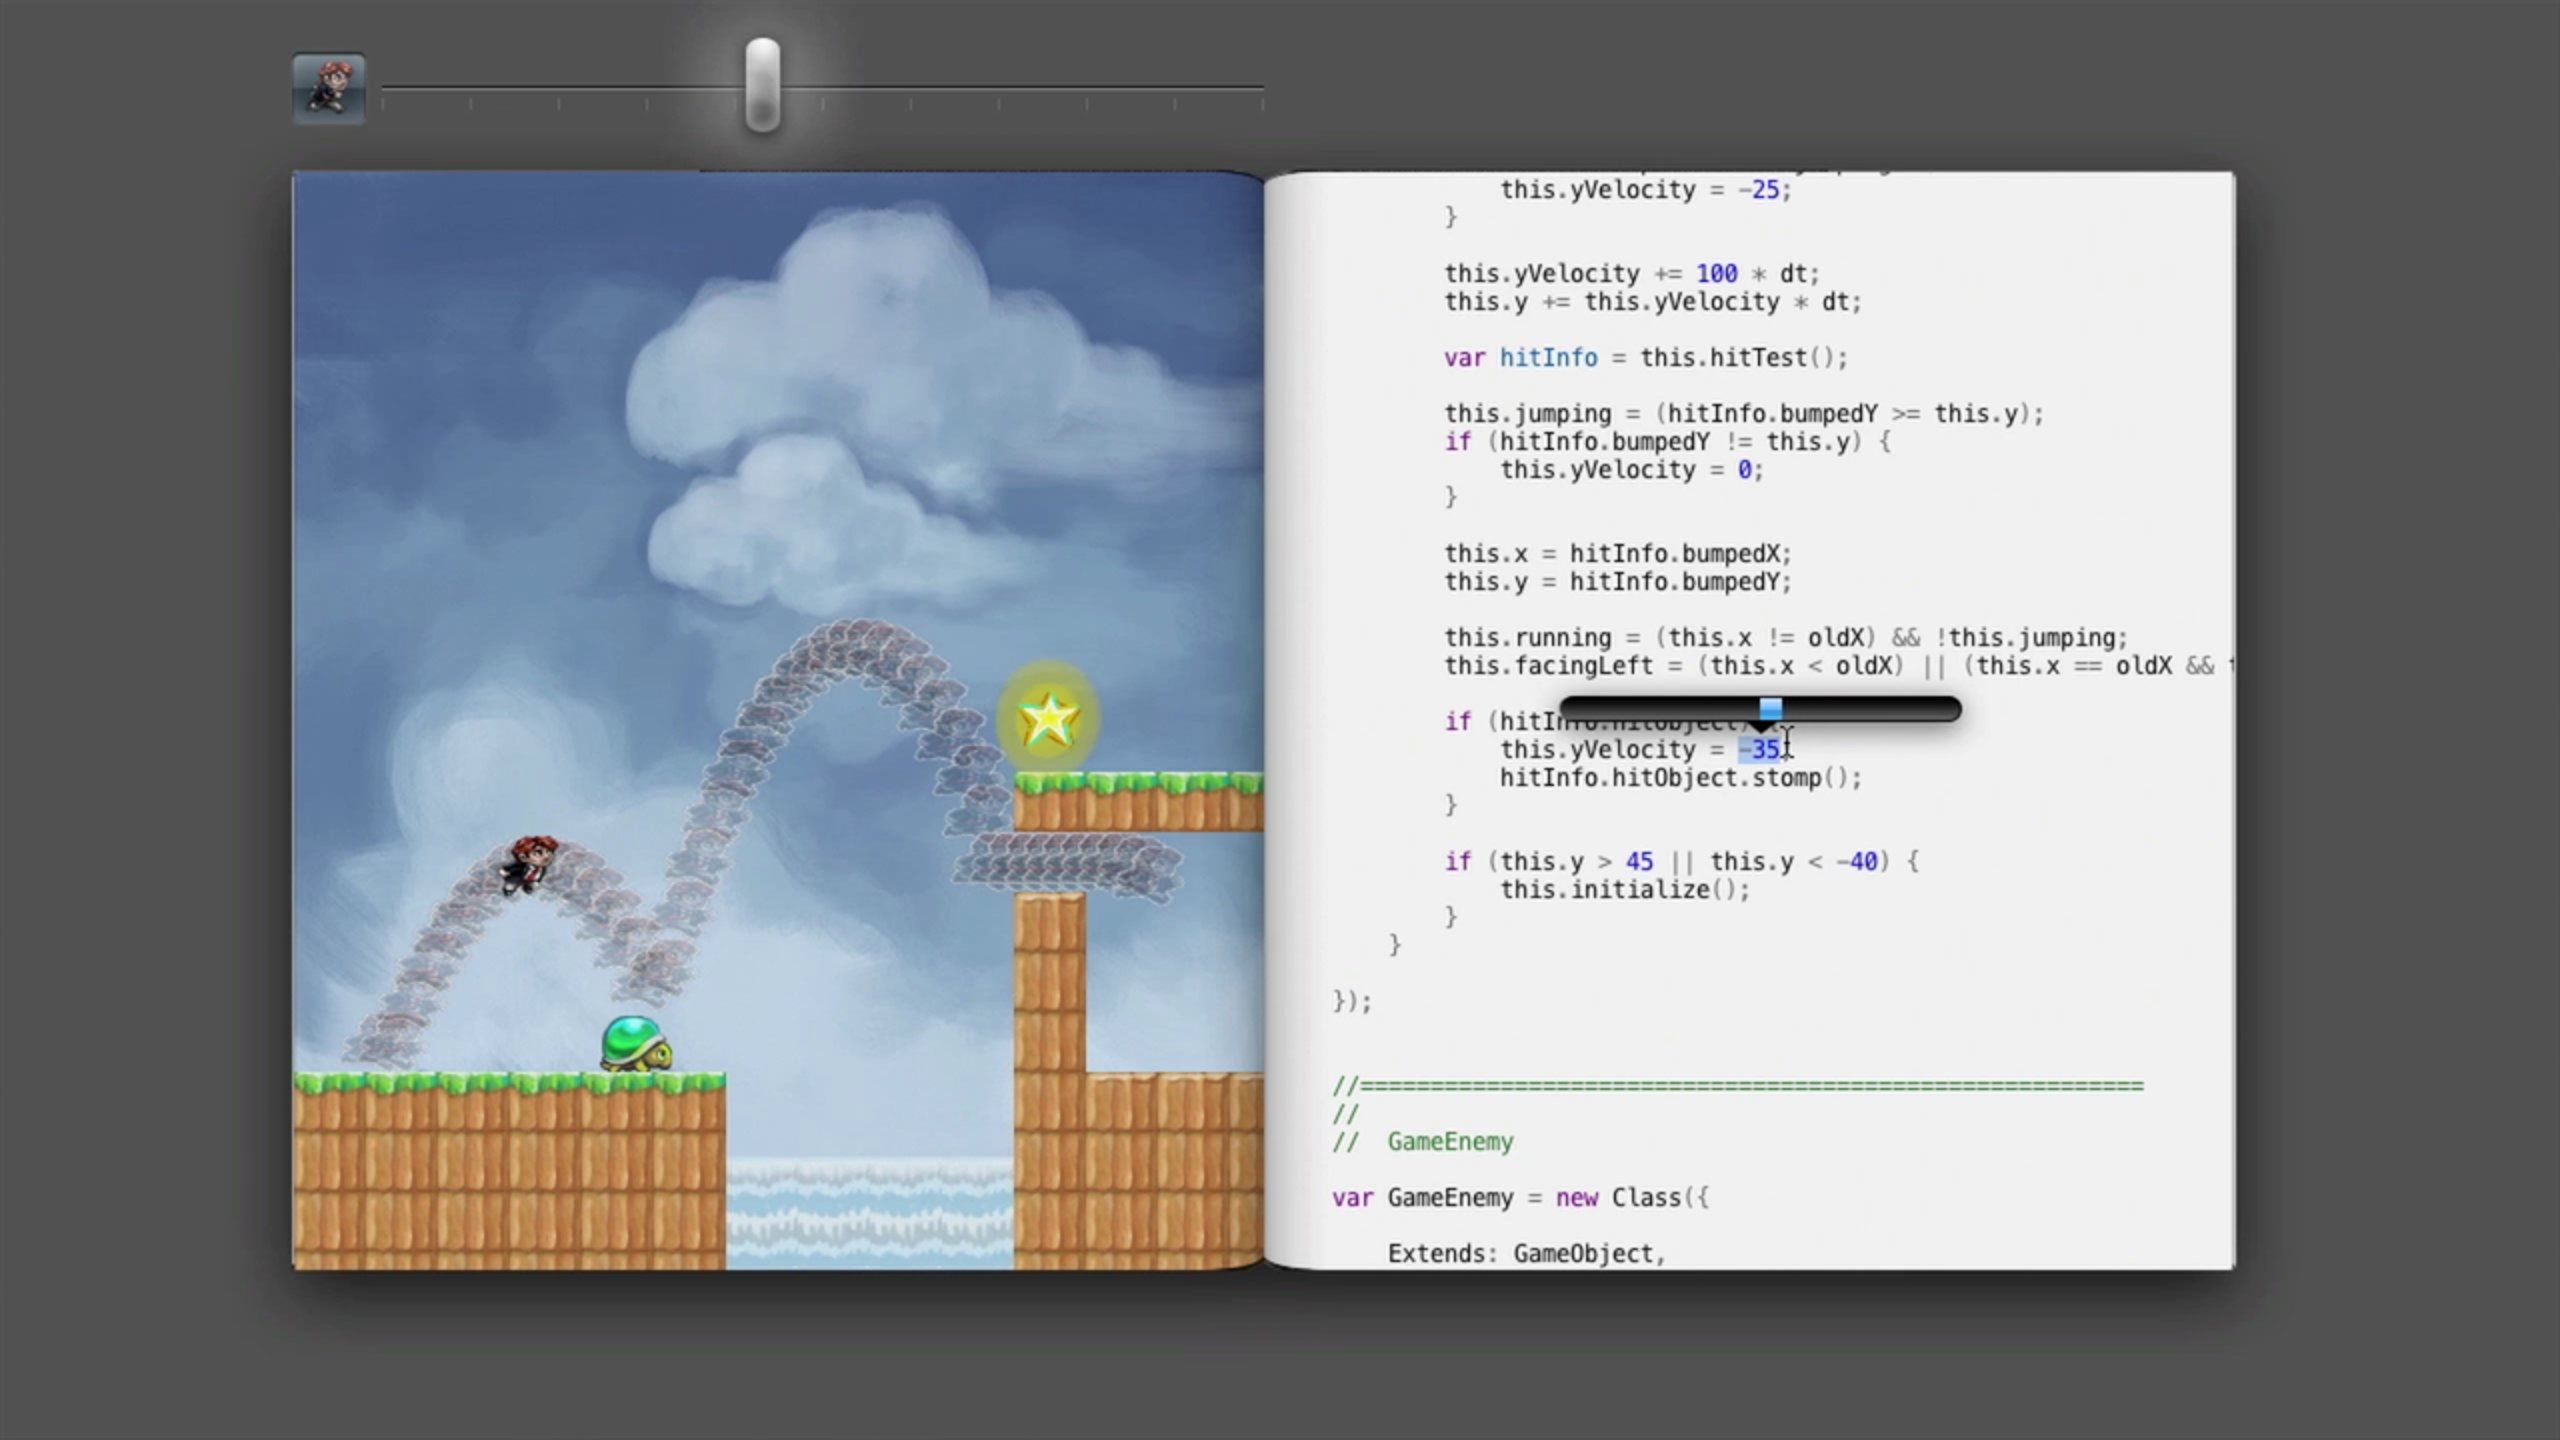
\includegraphics[scale=0.17, keepaspectratio]{bv.jpg}
  \caption{Screenshot from the talk \textit{Inventing on Principle} by
          Bret Victor (14:13) showing a prototypical live-coding
          environment.}
  \label{bv}
\end{figure}

This prototype showcases how the development of a 2D video game could
look like. As one can see the coding environment not only shows
the program code on the right hand side, but also shows a live and
\textit{running} version of the code on the left hand side.

So that whenever the user changes the value of, say the gravitational
attraction in the game, the effects of that change can immediately be
seen and experienced by playing with the Mario-like figure.
Unfortunately this still does not completely solve the problem of
having to emulate the actions of the computer as a programer because
what is the correct value for the gravitational attraction or velocity
in order for Mario to enter the little gap shown in Fig.\ref{bv}?
Although the change is immediately shown in the running program,
the programer would still have to use a trial-and-error approach
of figuring out the correct value by doing the jump in order to
see whether or not the chosen value works as expected.

In order to eliminate this tinkering and to close the feedback
loop even further, the environment features a \textit{time bar}
which records the history of the trajectory of the Mario-like
figure, as shown on the top of the screen.
So now the jump has to be recorded only once, and using
\textit{slide bars} in the code editor in order to sweep across
the value spectrum of a variable, the environment can show how
the trajectory of the jump would have looked like using the value
currently set in the code editor.

So now the programer can slide across different values, finding
the exact one that allows for the Mario-like figure to enter the litte gap
below the star, without having to manually trial-and-error different
values.
\newline

This concept of immediate feedback might seem alien in the context
of imperative languages and ahead-of-time compilation but is actually
not new in the context of functional programming.


Because functional programming languages won't easily allow
for state and base their concept of computation on the evaluation of
mostly side-effect free expressions, even Lisp \cite{commonlisp90}
featured what would later become known as a \textit{read-eval-print-loop}
(REPL), an interactive shell that
eagerly evaluated the expressions typed in by the user. Although
such an interactive shell does not immediately allow for the fluent
parameter tuning as shown by Bret Victor, it still delivers a more
immediate feedback loop than ahead-of-time compilation
and because of that allows for easier visualization of the current
user actions and the resulting state of the system.



